\documentclass[conference]{IEEEtran}
\usepackage{cite}
\usepackage{amsmath,amssymb,amsfonts}
\usepackage{algorithmic}
\usepackage{graphicx}
\usepackage{textcomp}
\usepackage{xcolor}
\def\BibTeX{{\rm B\kern-.05em{\sc i\kern-.025em b}\kern-.08em
    T\kern-.1667em\lower.7ex\hbox{E}\kern-.125emX}}

% Espacamento de floats reduzido para caber no limite de 5 paginas.
% Nao altera fonte nem margens do template IEEE.
\setlength{\textfloatsep}{8pt plus 2pt minus 2pt}
\setlength{\intextsep}{8pt plus 2pt minus 2pt}
\setlength{\dbltextfloatsep}{8pt plus 2pt minus 2pt}

\begin{document}

\title{A Latent World Model for Action-Conditioned Prediction in Interactive 2D Physics Environments}

\author{
\IEEEauthorblockN{Danilo César Tertuliano Melo}
\IEEEauthorblockA{
\textit{Universidade de Brasília} \\
Brasília, Brazil \\
daniloctmelo@gmail.com
}
\and
\IEEEauthorblockN{Felipe Lopes Gibin Duarte}
\IEEEauthorblockA{
\textit{Universidade de Brasília} \\
Brasília, Brazil \\
gibinf.duarte@gmail.com
}
\and
\IEEEauthorblockN{Matheus de Melo Fellet}
\IEEEauthorblockA{
\textit{Universidade de Brasília} \\
Brasília, Brazil \\
matheusmfellet@gmail.com
}
\and
\IEEEauthorblockN{Yuri Santana Lopes}
\IEEEauthorblockA{
\textit{Universidade de Brasília} \\
Brasília, Brazil \\
yuri03ysl@gmail.com
}
}

\maketitle

\begin{abstract}
World models offer a powerful paradigm for learning the internal representations and temporal dynamics of complex environments directly from high-dimensional sensory data. This paper presents a modular latent world model designed to predict the visual evolution of a two-dimensional physical simulation conditioned on external user interventions. To overcome the computational inefficiency and instability associated with direct pixel-space prediction, the proposed architecture decomposes the forecasting problem into visual compression, action embedding, multimodal fusion, and latent dynamics prediction. A Variational Autoencoder (VAE) is employed to compress individual $64 \times 64$ grayscale frames into a structured spatial latent space. Concurrently, an Action Encoder maps user interactions, specifically the instantaneous spawning of objects at given coordinates, into continuous latent vectors. These representations are combined via spatial broadcast fusion and fed into a transition predictor that estimates the subsequent latent state based on a stacked temporal history of past observations. Trained on a custom synthetic dataset generated via a 2D physics engine, the framework is evaluated on held-out episodes against trivial baselines and a reconstruction oracle. It predicts the next ball position more accurately than persistence and constant-velocity extrapolation in every test episode, and its predictions respond specifically and locally to user interventions, while capturing the direction of gravity-driven motion more reliably than its magnitude. This work provides a foundational approach for action-conditioned generative prediction in interactive physical environments.
\end{abstract}

\begin{IEEEkeywords}
World Models; Model-Based Reinforcement Learning; Action-Conditioned Prediction; Latent Dynamics; Synthetic Physics Environments.
\end{IEEEkeywords}

\section{Introduction}
\label{sec:introduction}

World models are generative models that aim to learn an internal representation of an environment and its temporal dynamics from observed experience. Instead of operating directly on high-dimensional sensory data, such as images or raw pixel observations, these models typically encode observations into a compact latent space in which the relevant spatial and temporal structure of the environment can be represented more efficiently. In this sense, a world model serves as an abstract simulator of the environment, allowing an agent or predictive system to estimate future states based on previous observations and actions \cite{ha2018world, hafner2019learning}.

In model-based learning, world models are particularly useful because they enable prediction, planning, and policy learning through imagined trajectories rather than relying exclusively on direct interaction with the real environment. Works such as PlaNet \cite{hafner2019learning} and Dreamer \cite{hafner2020dream} demonstrate that learning dynamics in latent space can support long-horizon reasoning from visual inputs, allowing agents to simulate possible futures and evaluate the consequences of actions before executing them. More recently, this paradigm has scaled towards overarching platforms for 'Physical AI', such as the Cosmos World Foundation Model \cite{agarwal2025cosmos}, which emphasizes the necessity of foundational models that inherently grasp complex physical laws and spatial dynamics. Therefore, in the context of this work, a world model can be understood as a latent generative model that learns the physical evolution of a simulated environment and predicts its next visual state conditioned on both the history of observations and external interventions.

The main contribution of this work is the development of a latent world model for predicting the visual evolution of a two-dimensional physical simulation conditioned on external user interventions. Unlike approaches that model future frames directly in pixel space, the proposed architecture separates the problem into visual compression, latent dynamics prediction, and visual reconstruction, enabling the system to learn a compact representation of the environment before modeling its temporal evolution. By combining a visual encoder, an action embedding module, a latent transition model, and a decoder, the proposed method investigates how physical interactions, such as gravity and collisions between circular bodies, can be learned in a structured latent space. This formulation provides a foundation for studying action-conditioned generative prediction in controlled physical environments and contributes to the broader development of world models capable of simulating future states from visual observations and interventions.

\section{Problem Formulation}
\label{sec:problem_formulation}

The objective of this work is to develop a generative model capable of predicting the evolution of a two-dimensional physical environment conditioned on external actions. More specifically, the goal is to estimate the next visual state of a simulation containing multiple balls subject to gravity and collisions, considering both the natural dynamics of the system and an intervention performed by the user.

The environment is represented as a temporal sequence of frames. Each frame corresponds to the complete visual state of the simulation at a given time step. Let \(x_t \in \mathbb{R}^{H \times W \times C}\) denote the observed frame at time \(t\), where \(H\) and \(W\) represent the height and width of the image, respectively, and \(C\) represents the number of channels. The input to the model consists of a temporal window containing the last \(k\) observed frames:

\begin{equation}
    X_t = \{x_{t-k+1}, x_{t-k+2}, \ldots, x_{t-1}, x_t\}.
\end{equation}

In addition to the visual sequence, the model receives an action \(a_t\), which is responsible for modifying the environment. In this work, actions correspond to the insertion of a new ball at specific coordinates in the scene. Thus, an action can be represented as a 4-dimensional vector:

\begin{equation}
    a_t = (v_{{\text{type}},t}, v_{{\text{obj}},t}, p^x_t, p^y_t),
\end{equation}

where $v_{{\text{type}},t} \in \{0.0, 1.0\}$ indicates the presence of an action (\texttt{mouse\_down} vs. \texttt{none}), $v_{{\text{obj}},t} \in \{0.0, 1.0\}$ encodes the type of object being introduced (\texttt{ball} vs. \texttt{none}), and $p^x_t, p^y_t \in [0,1]$ represent the normalized spatial coordinates of the interaction relative to the dimensions of the screen ($800 \times 600$). 

In the current experimental configuration, all physical and material properties of the system are kept strictly uniform. Specifically, the radius, mass, surface friction, and elasticity of the object remain constant across all instances and are thus omitted from the action embedding.

Due to the high dimensionality of the pixel space, direct modeling of the conditional distribution $P(x_{t+1} \mid x_{1:t}, a_t)$ is computationally expensive and prone to instability. Therefore, we adopt the fundamental premise of world models: the dynamics of the world can be represented in a more compact latent space.

The problem is therefore decomposed into three interdependent subproblems:

\subsection{Spatial Compression: Visual Perception}

The first step consists of reducing the dimensionality of the visual data. Instead of computing the dynamics directly over thousands of pixels, we seek to map each high-dimensional frame $x_t$ to a more compact and information-dense latent representation, denoted by $z_t$. To ensure a smooth and continuous latent space that facilitates the learning of temporal dynamics, this spatial compression is implemented using a Variational Autoencoder (VAE) \cite{kingma2013autoencoding}.

During its independent training phase, the VAE employs a probabilistic approach. The encoder function $E$ outputs the parameters of a multivariate Gaussian distribution, specifically the mean vector $\mu_t$ and the log-variance vector $\sigma_t^2$:

\begin{equation}
    (\mu_t, \log \sigma_t^2) = E(x_t).
\end{equation}

The network is optimized by sampling a latent vector $z_t$ using the reparameterization trick ($z_t = \mu_t + \sigma_t \odot \epsilon$, where $\epsilon \sim \mathcal{N}(0, I)$ and $\sigma_t = \exp(0.5 \log(\sigma_t^2))$). This formulation preserves end-to-end differentiability during training and encourages the latent space to remain smooth and continuous.

However, once the VAE is trained and deployed as a feature extractor for the World Foundation Model, we adopt a deterministic approach. To avoid injecting stochastic noise into the physics modeling, the latent representation of the frame is taken directly as the expected value of the distribution:

\begin{equation}
    z_t = \mu_t.
\end{equation} 

The purpose of this compression is to extract the fundamental characteristics of the scene, such as the spatial positions of the balls and the geometry of the environment, while discarding visual redundancies and noise. By stacking the latent representations of the last $k$ frames, we obtain the latent state history of the system, denoted by $Z_t$:

\begin{equation}
    Z_t = \{z_{t-k+1}, z_{t-k+2}, \ldots, z_{t-1}, z_t\}.
\end{equation}

\subsection{Latent Dynamics Prediction: World Modeling}

The core of the problem lies in learning the rules of physics, such as gravity, inertia, and collisions, in the latent space. In order for the model to understand user interventions, the action \(a_t\) is also mapped to a continuous numerical feature space through an embedding function, resulting in a representation \(e_t\):

\begin{equation}
    e_t = A(a_t),
\end{equation}

where \(A\) denotes the action embedding function.

The world model acts as a fully latent neural simulator. Each visual latent is fused with the action embedding of the same instant, so the window also carries the interventions applied while it was observed, $E_t = \{e_{t-k+1}, \ldots, e_t\}$. The transition function \(W\) receives this history and predicts the \emph{increment} of the latent state, the next state being obtained residually:

\begin{equation}
    \hat{z}_{t+1} = z_t + W(Z_t, E_t).
\end{equation}

Predicting the increment rather than the absolute state concentrates the learning signal on what changes between consecutive frames. It is in this stage that the system reasons about time and causality, determining the direction and velocity of the objects based on the provided temporal history.

\subsection{Visual Reconstruction of the Next Frame}

Finally, in order for the prediction to be interpretable and visually comparable to the real environment, the predicted latent state \(\hat{z}_{t+1}\) must be translated back into the original pixel space. This is performed by a decoder function \(D\), which maps the latent representation into a visible image:

\begin{equation}
    \hat{x}_{t+1} = D(\hat{z}_{t+1}).
\end{equation}

Thus, the problem formulation is defined in two main optimization stages. In the first stage, the focus is on optimizing the encoder \(E\) and decoder \(D\), so that the system can accurately represent the environment in the latent space and reconstruct it in the pixel space. In the second stage, once the spatial latent representation is well established, the focus shifts to the transition function \(W\), whose objective is to minimize the divergence between the predicted latent state \(\hat{z}_{t+1}\) and the true encoding of the next observed frame \(E(x_{t+1})\).

\section{Dataset}
\label{sec:dataset}

In order for the world model to learn how to represent the physics of the environment and respond to external commands, it was necessary to construct a more controlled dataset. The choice of synthetic data, rather than real-world videos, is justified by the need to isolate fundamental variables such as gravity, collision, and inertia from complex visual noise, including variable lighting, complex textures, and arbitrary occlusions, which could obscure the learning of purely mechanical dynamics.

\subsection{Simulation Environment}

The environment was built using the Pymunk 2D physics engine \cite{pymunk}, a Python interface for the Chipmunk2D library \cite{chipmunk2d}, which is capable of simulating fundamental mechanical properties in a deterministic manner. The basic scenario consists of a space with a floor and no walls, where physical interactions occur, as illustrated in Fig. \ref{fig:simulation_environment}.

\begin{figure}[!h]
    \centering
    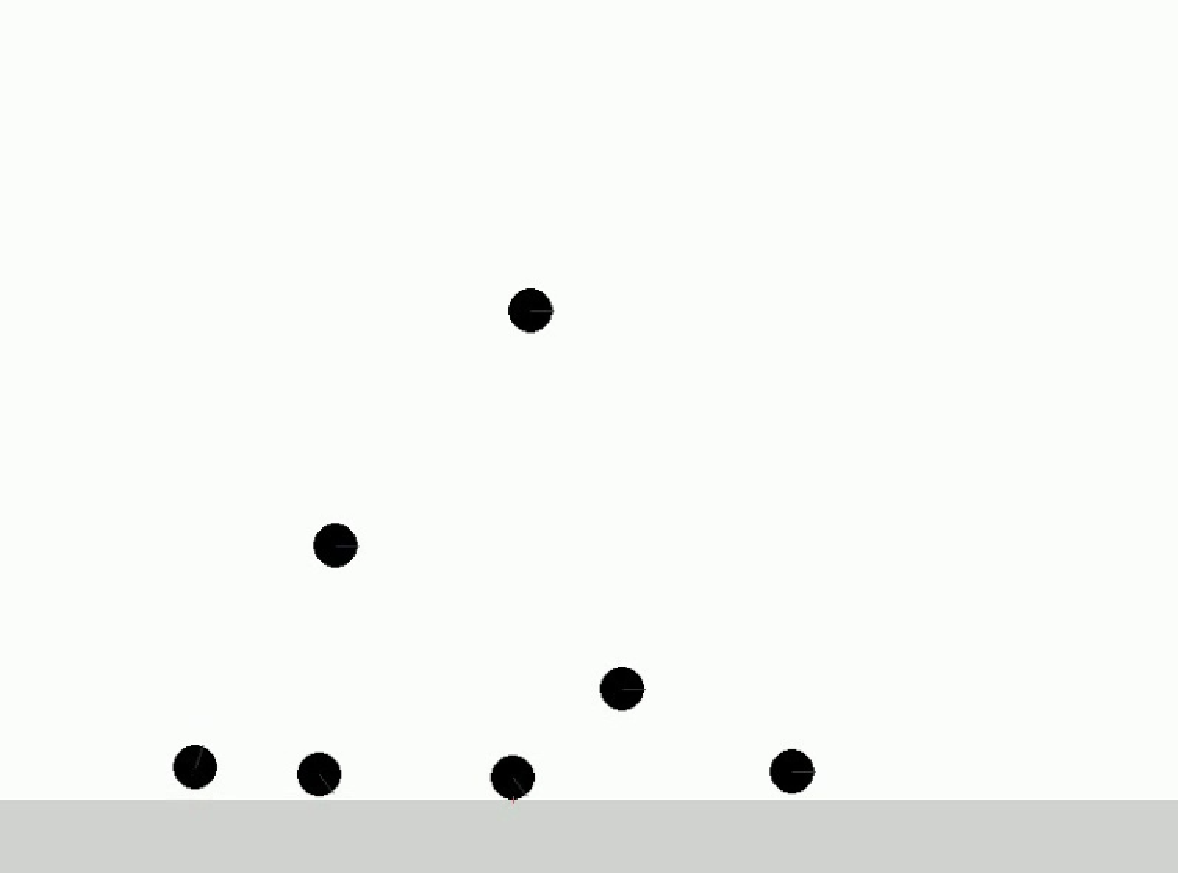
\includegraphics[width=\columnwidth]{figures/simulationEnvironment.pdf}
    \caption{Example frame from the simulated physical environment used for data generation. The scene contains multiple interacting objects whose dynamics are governed by the physics engine.}
    \label{fig:simulation_environment}
\end{figure}

The main dynamics of the environment involve circular objects that fall under the effect of gravity, collide with the floor and with each other, bounce with partial conservation of elastic energy, and eventually reach a resting state due to friction. The distinguishing feature of this environment is its interactivity: at any moment, an external intervention may occur in the form of a user ``click'' action, which instantly creates a new object at a specific coordinate on the screen, thereby altering the natural course of the simulation.

\subsection{Data Generation}

Data collection was automated through a set of procedural simulations, referred to as \textit{episodes}. Each episode consists of a short temporal sequence in which multiple actions are triggered at random times and positions, ensuring broad coverage of the state space. The generation process produces two synchronized data streams:

\begin{itemize}
    \item \textbf{Video:} The visual record of the simulation, rendered at a fixed rate of 60 frames per second (FPS). To reduce computational cost and focus on shape rather than color, the original frames, generated at higher resolutions such as \(800 \times 600\), are resized to \(64 \times 64\) pixels, converted to grayscale, and normalized to the interval \([0, 1]\).

    \item \textbf{Event Log:} A file in JavaScript Object Notation (JSON) format that records the exact time at which each action occurred and its corresponding properties. This log is used as input to automatically generate the video sequence.
\end{itemize}

An important detail in preparing these data for the temporal model is the construction of the frame history. Since the model requires a window of \(k\) frames, the initial time steps of the video, which do not have sufficient previous context, are padded by replicating the first available frame.

\subsection{Action Representation}

In a continuous simulation scenario, most frames occur without any external intervention. Therefore, the action representation needed to consistently handle both the moment of the click and the natural inertia of the environment.

Based on the event log, actions were extracted and aligned with the video frames using the timestamps and the fixed frame rate.

For frames in which the user does not perform any interaction, the system generates a \textit{Null Action}, represented by a zero vector corresponding to the absence of external intervention. This modeling choice is important because it teaches the model that, in the absence of an external action, it should only propagate the natural physics inferred from the previous frames.

\section{Proposed Model}
\label{sec:proposed_model}

The general architecture of this world model is organized as a modular pipeline designed to learn the dynamics of 2D physical scenes from simulations and structured actions, as illustrated in Fig.~\ref{fig:world_model_architecture}. Initially, scripts based on Pymunk and Pygame generate the physical scenarios, producing simulation videos and JSON files containing the actions executed over time. These videos go through a preprocessing stage, where they are converted into $64 \times 64$ grayscale frames. Then, a VAE is used to compress each frame into a compact visual latent representation, allowing the model to operate in a lower-dimensional space instead of working directly with image pixels.

\begin{figure}[!h]
    \centering
    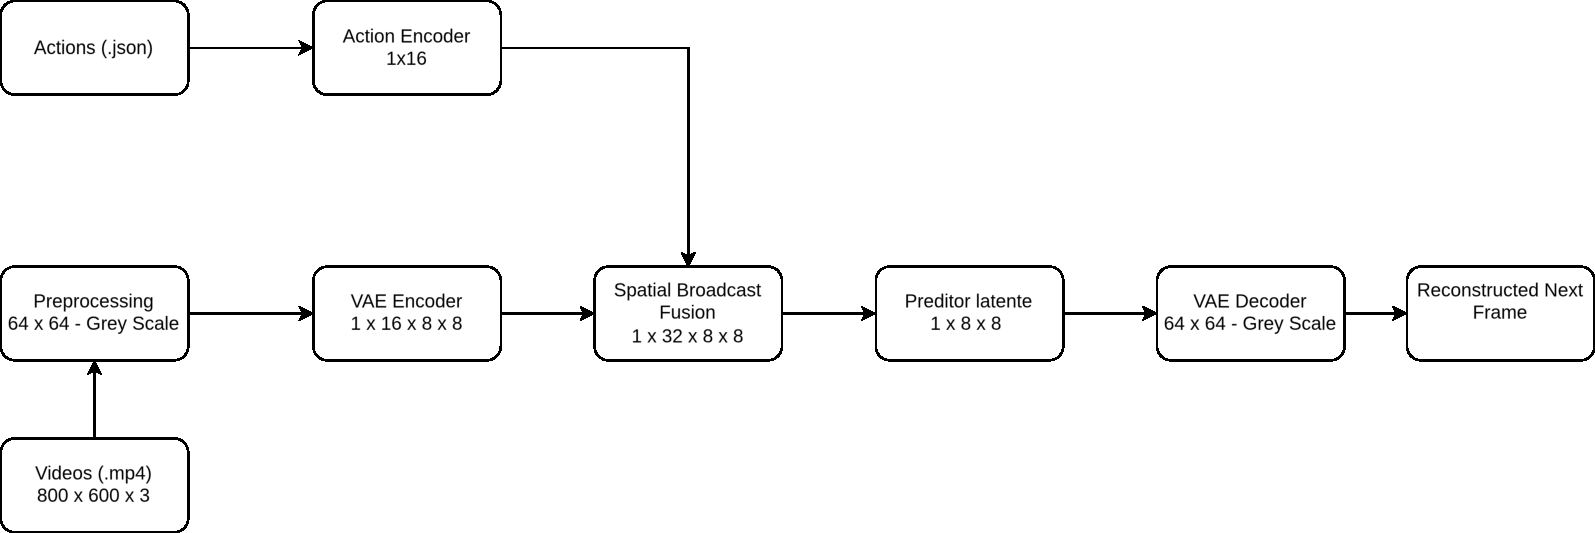
\includegraphics[width=\columnwidth]{figures/worldModel.pdf}
    \caption{Architecture of the proposed world model.}
    \label{fig:world_model_architecture}
\end{figure}

In parallel, each agent action is represented in a structured format using attributes such as action type, target object, and spatial coordinates. The action is encoded by an Action Encoder into a continuous latent vector, which is later combined with the visual representation through spatial broadcast fusion, inspired by the Spatial Broadcast Decoder architecture proposed in \cite{watters2019spatial}. In this process, the action embedding is replicated across the spatial dimensions of the visual feature map and concatenated with the visual features at every location. This enables the predictor to condition its representation of the scene dynamics on the agent's action while preserving the spatial structure of the scene. The resulting fused representation contains information about both the current state of the environment and the intervention performed by the agent.

From this representation, a predictor model learns to estimate the next visual state in latent space, which is then decoded by the VAE Decoder to reconstruct the next simulation frame. In this way, the architecture separates the problem into specialized components: visual representation, action representation, multimodal fusion, and prediction of the world's evolution.


\section{Experimental Setup}
\label{sec:experimental_setup}

Our experiments aim to verify two central hypotheses: (\textit{H1}) the model learns underlying physical dynamics (e.g., gravity, collisions) rather than merely memorizing trajectories; and (\textit{H2}) its predictions are genuinely conditioned by user interventions, independently of inertial cues already present in the visual context.

\subsection{Held-Out Evaluation Set}

Testing \textit{H1} against memorization requires unseen episodes, so 24 new ones were generated after training with the same engine, action distribution and rendering pipeline of Section~\ref{sec:dataset}, yielding $10{,}127$ evaluated transitions, $273$ conditioned by a click; regenerated frames are bit-identical to the original dataset. Following (1) and (5), the temporal window holds the $k$ most recent contiguous frames; sweeping $k \in \{1,2,4,6,8,10,12\}$ we adopted $k=6$, a single frame ($k=1$) degrading the skill score to $-0.803$ and confirming that the stacked history is what makes velocity estimable. Each action is assigned to the last frame that does \emph{not} yet contain the spawned ball, i.e. $\lceil t f_s \rceil - 1$ for an event at time $t$ with frame rate $f_s$: the object being absent from the visual context, any predicted response must originate from the action channel, which is what makes \textit{H2} meaningful.

\subsection{Baselines and Model Variants}

\textbf{Trivial baselines.} \emph{Persistence} ($x_{t+1} = x_t$) repeats the last frame; since objects come to rest due to friction it scores artificially high under pixel-level metrics, and any useful model must still beat it. \emph{Constant velocity} ($x_{t+1} = \text{clip}(2x_t - x_{t-1}, 0, 1)$) assumes uniform linear motion, failing on acceleration, elastic collisions and sudden insertions. Both are evaluated in two domains: \emph{pixel space}, as defined above, and the \emph{decoded domain}, where persistence becomes $\hat{z}_{t+1} = z_t$ and constant velocity extrapolates matched centroids, both undergoing the same reconstruction as the proposed model.

\textbf{Reconstruction oracle.} The \emph{VAE ceiling} decodes the true next latent, $\hat{x}_{t+1} = D(E(x_{t+1}))$: the lowest error attainable by any latent predictor coupled to this autoencoder. Since the oracle itself is far outperformed by pixel-space persistence, a comparison in pixel space cannot separate prediction from reconstruction; the decoded domain is therefore the primary reference for \textit{H1}, the pixel-space figures quantifying the cost of the autoencoder.

\textbf{Ablation.} \emph{No-Action} retains the complete architecture --- Action Encoder, Spatial-Broadcast Fuser and transition model all active --- but forces the action input to $\mathbf{0}$ at every step. Because no component is removed, any difference is attributable exclusively to the action signal, a direct test of \textit{H2}; by construction its action sensitivity is zero.

\subsection{Evaluation Metrics}

Image fidelity metrics (MSE, PSNR, SSIM) are combined with object-level physical ones, as pixel-level functions often fail to capture structural consistency and mass conservation. The \textbf{Centroid Position Error (CPE)} is the primary metric: balls are segmented by connected components under a contrast-adaptive threshold, their sub-pixel centroids matched by the Hungarian algorithm, and the mean Euclidean distance reported in pixels of the $800 \times 600$ screen. Since balls at rest are trivially predicted by persistence, we also report CPE restricted to \emph{moving} balls (displaced by more than $3$~px), and monitor mass conservation as the ratio of detected to true objects.

The \textbf{skill score} $1 - \mathrm{MSE}(\hat{z}_{t+1}, z_{t+1})/\mathrm{MSE}(z_t, z_{t+1})$ evaluates, in latent space, the divergence that the second training stage minimizes (Section~\ref{sec:problem_formulation}), and isolates the transition model from the decoder. \textbf{Action sensitivity} is the mean absolute difference between the frames predicted with and without the action, contrasted between click frames and non-click controls. Significance is assessed with paired Wilcoxon tests using the \emph{episode} as the experimental unit, since frames within an episode are correlated; intervals are obtained by bootstrap.

\subsection{Training and Inference Protocol}

Training follows the two-stage decomposition of Section~\ref{sec:problem_formulation}, the VAE converging before the temporal dynamics are learned. The transition function $W$ is a two-layer ConvLSTM with 64 hidden channels and two residual blocks, trained over $4$-step rollouts with an $L_1$ objective on the latent weighted $5\times$ on click frames, plus a decoded-frame term weighted $50\times$ on non-background pixels. Predictions are also evaluated in open-loop rollout, the model being fed back with its own output for up to $16$ frames while receiving only the future actions.


\section{Results}
\label{sec:results}

Both components converged --- VAE validation loss $293.52 \rightarrow 1.73$ over 200 epochs, action encoder $0.1795 \rightarrow 0.00013$ over 20 --- making the representations usable, but saying nothing about predictive ability, which the rest of this section addresses.

\subsection{Single-Step Prediction (H1)}

Table~\ref{tab:one_step} reports the error in predicting the immediate next state, in both evaluation domains.

\begin{table}[!t]
\caption{24 held-out episodes, CPE in screen pixels. \textbf{Top:} single step, with 95\% CI and fraction of objects recovered; the last two rows are computed directly in pixel space, the others in the decoded domain. \textbf{Bottom:} rollout by horizon $h$, and mean ball fall.}
\label{tab:one_step}
\centering
\scriptsize
\begin{tabular}{lccccc}
\hline
\textbf{Predictor} & \textbf{CPE} & \textbf{CI 95\%} & \textbf{CPE mov.} & \textbf{SSIM} & \textbf{det.} \\
\hline
Proposed model      & \textbf{24.69} & [24.08, 25.27] & 21.09 & 0.838 & 79.6\% \\
No-Action           & 25.13 & [24.49, 25.73] & 21.14 & 0.838 & 78.8\% \\
\textit{VAE ceiling}& \textit{25.76} & \textit{[25.13, 26.42]} & \textit{20.71} & \textit{0.839} & \textit{84.1\%} \\
Persistence         & 28.35 & [27.65, 29.01] & 24.01 & 0.833 & 83.7\% \\
Constant velocity   & 31.06 & [30.32, 31.80] & 25.67 & --- & 83.7\% \\
\hline
Persistence (px)    & 5.04 & [4.93, 5.18] & 8.46 & 0.972 & 99.8\% \\
Const. velocity (px)& 4.74 & [4.62, 4.87] & 7.88 & 0.974 & 99.8\% \\
\hline
\end{tabular}

\vspace{3pt}

\begin{tabular}{lcccccc}
\hline
$h$ & 1 & 2 & 4 & 8 & 12 & 16 \\
\hline
Proposed model      & \textbf{24.6} & \textbf{25.6} & \textbf{34.7} & \textbf{47.1} & \textbf{55.1} & \textbf{60.3} \\
Persistence         & 29.8 & 34.3 & 39.3 & 51.9 & 61.3 & 71.5 \\
Constant velocity   & 30.2 & 33.9 & 37.4 & 50.1 & 62.6 & 76.9 \\
\textit{VAE ceiling}& \textit{26.9} & \textit{25.0} & \textit{23.2} & \textit{29.9} & \textit{28.2} & \textit{22.6} \\
\hline
True fall (px)      & 7.5 & 8.9 & 12.9 & 18.8 & 23.0 & 28.2 \\
Predicted fall (px) & 2.0 & 3.5 & 5.7 & 7.2 & 7.8 & 10.6 \\
\hline
\end{tabular}
\end{table}

\textbf{Pixel space measures the autoencoder, not the prediction.} Evaluated directly on pixels, both trivial baselines outperform every latent method by a factor of five ($4.74$--$5.04$~px against $24.69$~px). The oracle settles the interpretation: decoding the \emph{true} next latent still yields $25.76$~px, so a predictor correct by construction also loses to copying the previous frame. The pixel-space gap therefore measures the cost of the autoencoder --- $7.4$~dB of PSNR and $16\%$ of the objects lost even in the oracle --- not the quality of the dynamics: in a predominantly static scene, pixel-level metrics reward reconstruction so heavily that prediction becomes unobservable.

\textbf{In the decoded domain the model beats every baseline.} It reduces the error to $24.69$~px against $28.35$ and $31.06$~px. Paired by episode the gain is $+3.69$~px (95\% CI $[3.10, 4.27]$) over persistence and $+6.35$~px (CI $[5.62, 7.03]$) over constant velocity, better in \textbf{all 24 episodes} in both comparisons ($p = 1.2 \times 10^{-7}$); restricted to moving balls, where persistence is no longer trivially correct, the gains remain $+2.97$ and $+4.57$~px, again in $100\%$ of episodes. In latent space the divergence minimized by the second training stage falls from $0.0776$ to $0.0724$, a skill score of $+0.066$, with a cosine of $+0.208$ between predicted and true increments.

The model operates at the level of the oracle ($21.09$ vs $20.71$~px on moving balls; the overall figures are confounded by the oracle's higher detection rate), so at one step the binding constraint is the decoder, not the dynamics, and the gain over the baselines is a \emph{lower bound} on the predictor's contribution.

\subsection{Open-Loop Rollout (H1)}

The lower half of Table~\ref{tab:one_step} reports the error when the model is fed back with its own predictions. It is more accurate than both baselines at \emph{all} 16 horizons, with reductions of $6.1$--$25.3\%$ over persistence and $21.6\%$ over constant velocity at $h = 16$. Since the oracle stays flat around $23$--$30$~px, the growth of the model error is attributable to the dynamics predictor, not to reconstruction --- the separation the single-step analysis could not provide.

The last two rows test gravity directly. The model does move the balls downwards --- persistence predicts a null displacement --- but recovers only $26$--$53\%$ of the true fall. With a ratio of $0.703$ between predicted and true latent increments, this supports a precise claim: the model learned \emph{that} bodies fall and in which direction, while underestimating \emph{how far} --- the signature of regression to the mean under an $L_1$ objective. Elastic collisions were not isolated by a dedicated metric and remain untested.

\subsection{Action Conditioning (H2)}

Running the model twice from an identical state, with and without the click, the predicted frames differ by $3.44 \times 10^{-3}$ on click frames against $4.41 \times 10^{-5}$ on the $10{,}039$ controls --- a ratio of $78.1\times$ with a large effect size (Cohen's $d = 3.02$, $p < 10^{-300}$, Mann--Whitney). The response is localized: the peak of the difference map falls within $100$~px of the clicked position in $85.0\%$ of events and within $200$~px in $90.1\%$, against a detector floor of $12.5$~px measured on the real video. Since the spawned ball is absent from the input frame by construction of the alignment, this cannot be explained by inertial cues, confirming \textit{H2}. The No-Action ablation attains nearly the same aggregate CPE (Table~\ref{tab:one_step}), which does not contradict this: only $2.7\%$ of frames carry a click, so the effect vanishes in an average.

\subsection{Limitations}

Three limitations follow from the measurements. The autoencoder binds visual quality: even decoding the true latent it misses $16\%$ of the objects, so image fidelity requires retraining the VAE, not the predictor. The predictor underestimates the magnitude of motion, its most actionable weakness. Lastly, it does not generalize across object scale: a checkpoint trained with one ball radius scores a skill of $-2.76$ on episodes with a different radius, the learned dynamics staying tied to the training environment.



\bibliographystyle{IEEEtran}
\bibliography{biblio}
\vspace{12pt}

\end{document}